%%%%%%%%%%%%%%%%%%%%%%%%%%%%%%%%%%%%%%%%%%%%%%%%%
%%%%%%%%%%%% chap: User Manual%%%%%%%%%%%%%%%%%
%%%%%%%%%%%%%%%%%%%%%%%%%%%%%%%%%%%%%%%%%%%%%%%%%

\chapter{User Manual}\label{chapter:chap5}

\section{Main Menu}\label{sect:Main Menu}

\begin{figure}[htp]
    \centering
    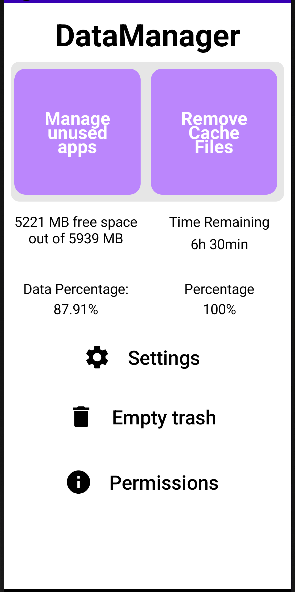
\includegraphics[width=200pt]{mainmenu.png}
    \caption{Main Menu Screen}
    \label{fig: Main Menu Screen}
\end{figure}

In Figure 5.1 we can see the main menu screen of the application, the user is greeted with a menu consisting of 5 buttons, each with its own unique functionality. The first time the user opens the application, some default settings will be placed and stored in the database, with the theme being a light one, the language being English, and no permissions being given by default, the app waiting for the user to give them when he either enters the cache screen and tries to analyze for residual files when he tries to enter the manage unused apps, or when he tries to press on the empty trash button. Each time the user tries one of these actions, the application will see if the permissions were granted, if so, the application can continue. 

\section{Permissions Menu}\label{sect:Permissions Menu}

\begin{figure}[htp]
    \centering
    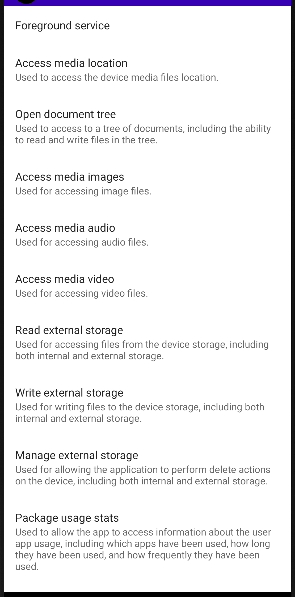
\includegraphics[width=200pt]{permissions.png}
    \caption{Permissions Menu Screen}
    \label{fig: Permissions Menu Screen}
\end{figure}

Figure 5.2 shows the screen that pops up when the user presses the permissions button in the main menu. The screen is used for telling the user what is he about to give his consent to, and what each of the required permissions is about. The permissions are as follows: 

    - Access media location;

    - Access foreground services;

    - Access image, video, and audio files;

    - Read both internal and external storage;

    - Write on both internal and external storage;

    - Manage both internal and external storage;

    - Package Usage stats, which allows the app to access information about the app usage;

    - Query all packages, which allows the app to gather information on all installed packages on the device;

\section{Settings Menu}\label{sect:Settings Menu}

\begin{figure}[htp]
    \centering
    \begin{minipage}{0.45\textwidth}
        \centering
        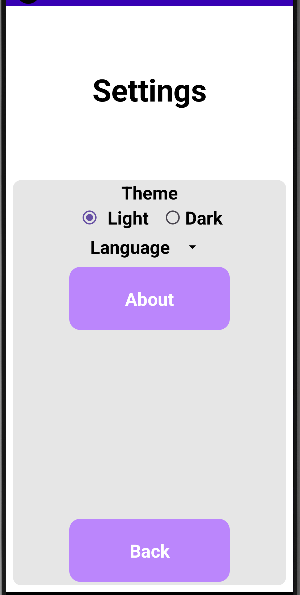
\includegraphics[width=205pt]{SettingsMenu.png}
        \caption{Light Settings Menu}
        \label{fig: Light Settings Menu}
    \end{minipage}\hfill
    \begin{minipage}{0.45\textwidth}
        \centering
        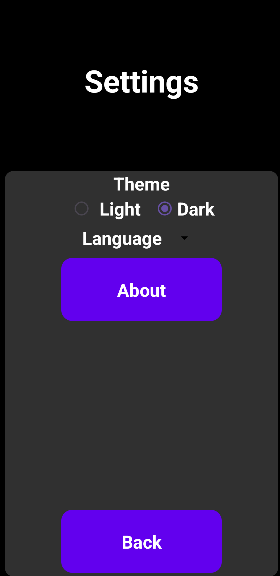
\includegraphics[width=200pt]{darksettingsmenu.png}
        \caption{Dark Settings Menu}
        \label{fig: Dark Settings Menu}
    \end{minipage}
\end{figure}
\newpage
Figures 5.3 and 5.4 showcase the settings menu and its buttons, those being the 2 radio buttons for the theme of the app, consisting of a Light and Dark mode, the Language dropdown menu used for changing the language of the application, the About button that opens the about menu which offers some additional information on what the app is about and the back button for going back to the main menu screen. The preferences set by the user are saved in the Firebase Realtime Database. 

The following 2 figures, Figures 5.5 and 5.6, showcase the changes in the layout of the application when the user chooses to change the language from English to Romanian, each element of text being changed to the other language seamlessly.

\begin{figure}[htp]
    \centering
    \begin{minipage}{0.45\textwidth}
        \centering
        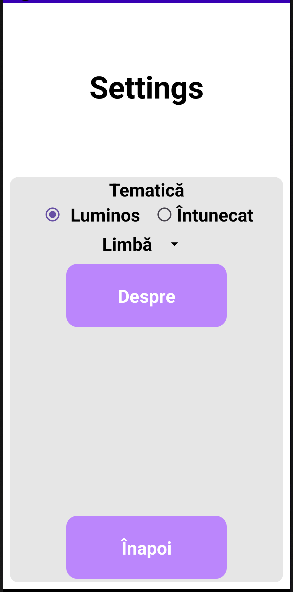
\includegraphics[width=205pt]{romanian.png}
        \caption{Settings Menu with Romanian text}
        \label{fig: Settings Menu with Romanian text}
    \end{minipage}\hfill
    \begin{minipage}{0.45\textwidth}
        \centering
        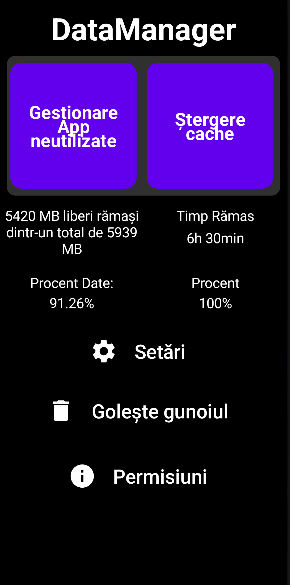
\includegraphics[width=200pt]{romanianmainmenu.png}
        \caption{Main Menu with Romanian text}
        \label{fig: Main Menu with Romanian text}
    \end{minipage}
\end{figure}
\newpage

\section{Cache Screen}\label{sect:Cache Screen}

\begin{figure}[htp]
    \centering
    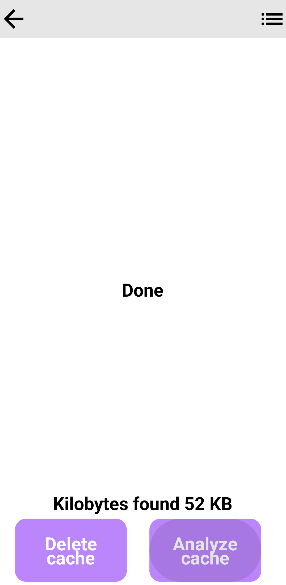
\includegraphics[width=200pt]{cachedeletionscreen.png}
    \caption{Cache Remover Screen}
    \label{fig: Cache Screen}
\end{figure}

Figure 5.7 showcases the Cache Deletion Screen. Here the user has several options, first, up top, is the back button on the top left, marked by a left-pointed arrow, and the second, top right, the filter settings, represented by the three lines, which, when pressed, takes the user to the filter settings of the app.

On the other hand, at the bottom, the other two buttons, analyze and delete, do pretty much what the name suggests, starting a general scan of the storage of the phone for signs of the type of files the user has selected, while the delete button removes said files. When clicking the buttons, a progress bar will appear showcasing that the search is still ongoing, and, after the search is done, 2 new texts appear, one saying "Done", and the other showcasing the amount of memory found/deleted.


\newpage
\begin{figure}[htp]
    \centering
    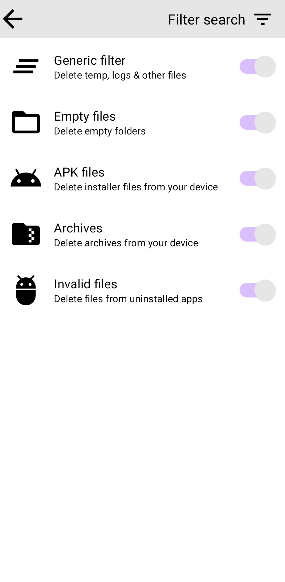
\includegraphics[width=200pt]{filter menu.png}
    \caption{File Filter Menu}
    \label{fig: File Filter Menu}
\end{figure}

The above figure, 5.8, presents the filter search settings menu that the app includes in the cache deleting screen. Here the user can switch on and off what type of files he or she wants to delete, those types ranging from temp, and logs to empty folders and leftover files, the screen shows for each file type a short description of what exactly the app will look for.

Each option is saved in a separate collection from the user preferences one, in Firebase Realtime Database, so that the user doesn't have to re-select what type of file he wants to get rid of each time they re-enters the application.

\newpage
\section{Unused App Screen}\label{sect:Unused App Screen}

\begin{figure}[htp]
    \centering
    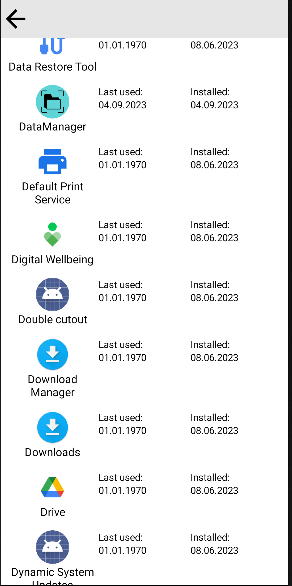
\includegraphics[width=200pt]{UnusedAppMenu.png}
    \caption{Unused App Menu}
    \label{fig: Unused App Menu}
\end{figure}

The Unused App Screen, shown in the 5.9 figure, lists all applications present in the users' application list, being ordered in an alphabetical manner. 

The list of applications showcases in three columns the name and icon, the last time they were used, and the date that the applications were installed. For applications that were never used or have been installed by default, usually, a generic date will be displayed, usually the Unix epoch, more specifically 1.01.1970, while apps that were actually used and installed by the user will showcase the correct dates.

\newpage
\begin{figure}[htp]
    \centering
    \includegraphics[width=200pt]{AppInfo.png}
    \caption{App Info}
    \label{fig: App Info}
\end{figure}

The user has the option in the Unused App Screen to click on any of the listed applications and be transported to the general App Info screen, as seen in the 5.10 figure. Here the user has the liberty to do whatever they want. It's up to them if they want to delete, force stop, set new preferences, and so on for the app they clicked on, or they can just as well leave it alone.

When done with the app, the user can go back to the DataManager app by simply clicking on the above arrow, the user being transported back to where they were on the app list.
\newpage
\begin{figure}[htp]
    \centering
    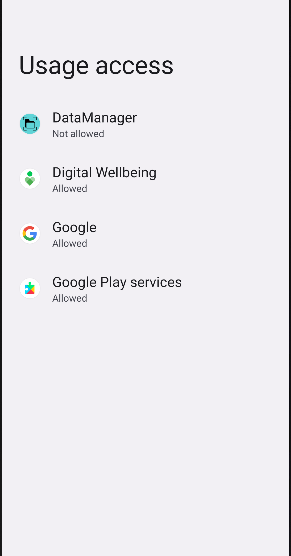
\includegraphics[width=200pt]{UsageAcess.png}
    \caption{Usage Access}
    \label{fig: Usage Access}
\end{figure}


The last figure, 5.11, represents the usage access screen that asks the user for the above-mentioned permissions, found in Figure 5.2. What the user needs to do here is simple, he needs to click on the DataManagerApp, and switch on the permission for usage access. 

After closing the usage access screen, another one will pop up that asks for access to all files in the system. Again, the user just has to click on the app, in the list, and check on the switch for storage permissions. After switching on the two options, the user will be able to use the functionalities of the application.
\newpage
